
%(BEGIN_QUESTION)
% Copyright 2010, Tony R. Kuphaldt, released under the Creative Commons Attribution License (v 1.0)
% This means you may do almost anything with this work of mine, so long as you give me proper credit

The following motor control ``bucket'' has a problem.  When the ``Start'' button is pressed, the motor refuses to start:

$$\includegraphics[width=15.5cm]{i04523x01.eps}$$

Using your digital voltmeter, you measure 54 volts AC between TP11 and Ground when the ``Start'' switch is pressed, but 0 volts between the same points when the switch is released.  From this information, identify two possible faults (either one of which could account for the problem and all measured values in this circuit).  The circuit elements you identify as possibly faulted can be wires, traces, and connections as well as components.  Be as specific as you can in your answers, identifying both the circuit element and the type of fault.

\begin{itemize}
\goodbreak
\item{} Circuit elements that are possibly faulted
\item{1.}
\item{2.} 
\end{itemize}

Also, explain why a bad (open) connection between L2 and chassis ground would {\it not} account for this circuit's problem.

\vfil 

\underbar{file i04523}
\eject
%(END_QUESTION)





%(BEGIN_ANSWER)

This is a graded question -- no answers or hints given!

%(END_ANSWER)





%(BEGIN_NOTES)

Although we expect to see voltage between TP11 and ground when the ``Start'' pushbutton is pressed, it ought to be more than the 54 volts we're measuring in this scenario.  This points to either a source with insufficient voltage, a partial (high-resistance) open fault between the test points and the source, or a partial (low-resistance) shorted fault that loads down the source voltage to much less than it ought to be.

\vskip 10pt

Note: the following answers are not exhaustive.  There may be more circuit elements possibly at fault and more circuit elements known to be functioning properly!

\begin{itemize}
\item{} Circuit elements that are possibly faulted
\item{1.} High-resistance connection at fuse 1 or fuse 2
\item{2.} Dirty (high-resistance) contacts in Start switch contacts
\item{3.} Dirty (high-resistance) contacts in Stop switch contacts
\item{4.} Partially shorted secondary winding in transformer
\item{5.} Abnormally low 3-phase supply voltage (i.e. a ``brownout'' condition)
\end{itemize}

\vskip 10pt

One popular but incorrect suggestion is that the safety ground connection at L2 might account for the low voltage reading taken by the voltmeter.  However, we may eliminate this possibility by considering the fact that the motor refuses to start.  Even with the ground connection failed open, a complete circuit would still exist to energize the contactor coil (and keep it latched) when the ``Start'' button is pressed, so the motor would start just fine even with an open ground connection at L2.

%INDEX% Troubleshooting review: electric circuits

%(END_NOTES)


